\documentclass[11pt]{article}
\usepackage[margin=1in]{geometry}
\usepackage{amsmath,amssymb,amsthm,booktabs,graphicx}
\usepackage[colorlinks=true,linkcolor=blue,urlcolor=blue,citecolor=blue]{hyperref}
\newtheorem{theorem}{Theorem}[section]
\newtheorem{proposition}[theorem]{Proposition}
\newtheorem{corollary}[theorem]{Corollary}
\newtheorem{remark}[theorem]{Remark}
\newcommand{\R}{\mathbb R}
\newcommand{\E}{\mathbb E}
\newcommand{\ip}[2]{\langle #1,#2\rangle}
\newcommand{\F}[1]{\lVert #1\rVert_{\mathrm F}}
\newcommand{\nuc}[1]{\lVert #1\rVert_*}
\newcommand{\op}[1]{\lVert #1\rVert_{\mathrm{op}}}
\newcommand{\ent}[1]{\lVert #1\rVert_1}
\newcommand{\sgn}{\operatorname{sign}}
\newcommand{\rank}{\operatorname{rank}}
\newcommand{\pos}[1]{[#1]_+}
\title{Convergence bounds that distinguish Fanions:\\rank, step budget, curvature, and noise}
\author{Research attempt for the Neon repository}
\date{21 October 2026}
\begin{document}
\maketitle

\begin{abstract}
Equal exponents in worst-case convergence bounds do not imply equal finite
iteration performance. We derive two loss lower bounds for exactly the
quadratic class used in the manuscript: one for the rank of the accumulated
update, and a stronger one for its accumulated nuclear norm. The latter gives
a necessary iteration count proportional to $1/k$ at the same learning rate,
independently of momentum. On a fresh $500\times500$ draw from the specified
distribution, Neon requires at least 65,172 iterations at learning rate 0.007
to reach loss 0.001. This is an analytic lower bound, not a training run.
We also give convergence upper bounds retaining the singular spectrum,
curvature, and oracle error, and quantify the robustness of F-Muon and S-Muon.
A saved-log audit supports the Muon--Neon spectral comparison but also
falsifies the sufficiency of a Frobenius-only explanation for all methods.
These results explain a concrete mechanism behind Neon's poor performance;
they do not establish the complete CIFAR/LLM accuracy ordering.
\end{abstract}

\section{What is established, and what is still missing}

\paragraph{Continuation across all ranks.}
The companion \path{fanion_followup.pdf} extends this first attempt with a
unified plain/F/S-Fanion convergence bound, tracking for the actual code's
Nesterov convention, stronger singular-budget obstructions, solvable rank
flows, and a saved quadratic trajectory audit. It also identifies a
different learning-rate schedule for F-Fanion-10 in the current benchmark
source. The scalar nuclear lower bounds below remain valid; the follow-up
retains additional operator and spectral information to strengthen them.

\paragraph{The strongest result for the manuscript.}
Theorem~\ref{thm:barriers} applies to its synthetic objective without assuming
gradient accuracy, particular momentum coefficients, or an oracle trajectory.
It bounds \emph{loss}, and gives a large obstruction for Neon at the learning
rates actually used. A separate example gives a tight $r/k$ iteration
separation between Fanion-$k$ and Muon even with arbitrary learning rates.

\paragraph{A conditional explanation for deep learning.}
The appropriate comparison is the true gradient's projection onto the update,
squared, divided by curvature along that update. The singular spectrum already
distinguishes Muon from Neon in most saved CIFAR snapshots. Momentum error,
directional curvature, and the effect of weight normalization have not been
recorded in those snapshots. Their values are needed for a complete
explanation of the actual algorithms. In particular, our Frobenius surrogate
incorrectly favors F-Neon over Muon; we report this failure rather than
interpreting every bound as evidence for the desired ordering.

\paragraph{The experimental premise needs qualification.}
Section 5.1 of \path{jota_submission/main.tex} reports F-Muon and S-Muon
reaching the synthetic loss threshold in 910 and 890 iterations, versus 1060
for Muon. Their real-task performance is close to Muon's. Thus the target is
Muon being much better than the low-rank Fanions and comparable to its full-rank
hybrids, with possible reversals among the latter.

\paragraph{Status of originality.}
The ingredients are classical: the descent lemma, best rank approximation,
norm inequalities, and gradient-estimator tracking. The Muon specialization
of the descent calculation is already present in the literature. The
contribution of this attempt is their explicit specialization to Fanions,
the finite learning-rate obstruction for the manuscript's quadratic, the
hybrid comparison, and the audit. No claim of priority or a complete
literature survey is made.

\section{Literature check as of 21 October 2026}\label{sec:literature}

The statement that no relevant theory has improved is too strong.
\begin{itemize}
\item Kovalev and Borodich, \emph{Non-Euclidean SGD for Structured
Optimization}, v2, 22 June 2026~\cite{structured}, obtain improved guarantees
under structured Hessian and gradient-noise assumptions. Their Assumption 5
puts the relevant bounding operators in a common subspace with an
order-preserving projection and algebraic closure properties. Theorems 1--3
cover momentum, extrapolation, and momentum variance reduction. These are
conditional structural improvements; they do not assert a universal ordering
of Muon, Neon, and all hybrids. This paper is already in the local bibliography.
\item Shen et al., \emph{On the Convergence Analysis of Muon}, v3, 28 July
2026~\cite{shen}, retain matrix smoothness and Hessian information. Their
proofs explicitly contain the Muon decrease
$\nuc{G}^2/(2rL)$ and a spectral-smoothness alternative. A spectrum-dependent
Muon comparison is therefore not new by itself. Our use of all $k$, hybrid
directions, and a common Frobenius stopping metric makes the comparison more
direct for this manuscript.
\item Nagashima and Iiduka, v3, 5 March 2026~\cite{nagashima}, claim sharper
iteration rates, including schedules with increasing batches. However,
Corollary 3.1 defines $D_1=\Delta/\eta+C_3/(1-\beta)$: its $D_1/T$ term cannot
be treated as uniform when $\eta$ depends on $T$. The displayed assertion
with $\eta=1/T$ is contradicted by noiseless scalar $f(x)=x^2/2$, $x_0=2$,
$\beta=0$: normalized steps of size $1/T$ leave $x_t\geq1$ through $T$ steps.
The script reproduces this check. We do not rely on those claimed faster
rates. Increasing batch size also changes oracle cost.
\item Ma et al., \emph{Schattor}, June 2026~\cite{schattor}, study a Schatten
family and state dimension-free stationarity guarantees in their abstract.
This is further relevant work after the manuscript's main 2025 references;
an abstract claim alone is not a proof of the requested optimizer ordering.
\item Kovalev's trust-region framework~\cite{trust} and Gluon~\cite{gluon}
remain relevant foundations. General norm guarantees must retain their
geometry and use the same accuracy metric before numerical rates are compared.
\end{itemize}
In particular, improved constants under structure, faster rates under extra
regularity, and a change from iteration count to total gradient evaluations
are different assertions. None implies that one norm is best on every smooth
objective.

\section{Notation and the common comparison metric}

Let $f:\R^{m\times n}\to\R$ be differentiable and bounded below by $f_*$,
$r=\min(m,n)$, $G=\nabla f(X)$, and
$G=U\operatorname{diag}(\sigma_1,\ldots,\sigma_r)V^\top$, with decreasing
nonnegative singular values. Define
\[
 S_k(G)=\sum_{i=1}^k\sigma_i(G),\qquad
 D_k(G)=\sum_{i=1}^k u_i v_i^\top.
\]
We take only positive singular directions if fewer than $k$ are nonzero, and
set $D_k(0)=0$. When $\rank G\geq k$,
\begin{equation}\label{eq:fanion-identities}
 \ip{G}{D_k(G)}=S_k(G),\quad \F{D_k(G)}^2=k,\quad
 \nuc{D_k(G)}=k,\quad\op{D_k(G)}=1.
\end{equation}
Fanion-$k$ uses $X^+=X-\gamma D_k(H)$, where $H$ may be a stochastic gradient
or a momentum matrix. Neon has $k=1$; Muon has $k=r$.

All stationarity comparisons below use the \emph{same} $\F{\nabla f}$, and all
loss comparisons use the same $f-f_*$. Comparing an $\epsilon$-spectral norm
gradient for Neon with an $\epsilon$-nuclear norm gradient for Muon is not a
common stopping criterion.

For the hybrids write $a=\alpha$, $b=1-\alpha$ and retain the manuscript's
actual direction coefficient $\eta$:
\begin{equation}\label{eq:hybrids}
 D_{F,k}(H)=aD_k(H)+b\frac{H}{\F H},\qquad
 D_{S,k}(H)=aD_k(H)+b\eta\sgn(H).
\end{equation}
Positive scalar rescaling of an entire direction is absorbed by the learning
rate. Rescaling only one summand changes a hybrid's direction.

\section{A loss obstruction for exactly the manuscript's quadratic}

Consider, including a possible shift $Z$,
\begin{equation}\label{eq:quadratic}
 f(X)=\frac12\F{M^{1/2}(X-Z)N^{1/2}}^2,\quad M,N\succeq0,
 \qquad L=\op M\op N.
\end{equation}
The manuscript uses $Z=0$. Define $E_0=M^{1/2}(X_0-Z)N^{1/2}$ and
$s_j=\sigma_j(E_0)$. No inverse of $M$ or $N$ is required.

\begin{theorem}[Rank and nuclear-norm obstructions]\label{thm:barriers}
Let $X_{t+1}=X_t-\gamma_t A_t$, where $\rank A_t\leq k$ and
$\nuc{A_t}\leq k$, with $\gamma_t\geq0$. Then, for every $T$,
\begin{align}
 f(X_T)&\geq \frac12\sum_{j>kT}s_j^2,
 \label{eq:rank-bound}\\
 f(X_T)&\geq\frac{1}{2r}
  \pos{\nuc{E_0}-\sqrt L\,k\sum_{t<T}\gamma_t}^{\!2}.
 \label{eq:nuclear-bound}
\end{align}
The rank bound only needs the rank assumption. The nuclear bound only needs
the nuclear-norm assumption.
\end{theorem}
\begin{proof}
Write $E_T=E_0-R_T$, where
$R_T=\sum_{t<T}\gamma_t M^{1/2}A_tN^{1/2}$. Rank subadditivity gives
$\rank R_T\leq kT$. The best approximation of $E_0$ by a matrix of rank at
most $kT$ in Frobenius norm has squared error $\sum_{j>kT}s_j^2$, proving
\eqref{eq:rank-bound}. This follows directly by truncating the SVD and its
standard optimality characterization.

Also, $\nuc{M^{1/2}A_tN^{1/2}}\leq\sqrt L\nuc{A_t}\leq\sqrt Lk$.
The triangle inequality implies
$\nuc{E_T}\geq\pos{\nuc{E_0}-\sqrt L k\sum_{t<T}\gamma_t}$.
Finally, $\nuc{E_T}\leq\sqrt r\F{E_T}$ and $f(X_T)=\F{E_T}^2/2$.
\end{proof}

\paragraph{Why this handles momentum.}
The theorem permits any $A_t$ satisfying the two constraints. Hence it covers
exact rank-$k$ Fanion updates from any heavy-ball or approximate Nesterov
matrix, noisy gradients, adversarial singular-vector choices, and arbitrary
learning-rate schedules. Momentum can change the selected singular
directions; it does not increase the rank or nuclear norm of a single
rank-$k$ partial isometry.

\begin{corollary}[Necessary iterations at a constant learning rate]
If $f(X_T)\leq\epsilon$ and $\gamma_t=\gamma>0$, then
\begin{equation}\label{eq:necessary-T}
 T\geq
 \frac{\pos{\nuc{E_0}-\sqrt{2r\epsilon}}}{\sqrt L\,k\gamma},
 \qquad
 \sum_{j>kT}s_j^2\leq2\epsilon.
\end{equation}
More generally, the first inequality bounds $\sum_t\gamma_t$.
\end{corollary}

\subsection{A numerical consequence at the manuscript's scale}

We generated a fresh draw with $m=n=500$, independent uniform eigenvalues of
$M,N$ in $(0,1)$, and Gaussian $X_0$ with standard deviation $0.1$, interpreting
$\mathcal N(0,0.01)$ as variance $0.01$. Working in the eigenbases preserves
the Gaussian distribution and these bounds. This is not the original
PyTorch seed or a rerun of the published training curves.

The draw gives $f(X_0)=337.933502$, $\nuc{E_0}=456.207241$, and a necessary
approximation rank of 484 to reach $\epsilon=0.001$. At $\gamma=0.007$,
\eqref{eq:necessary-T} gives the following integer lower bounds:
\begin{center}
\begin{tabular}{lrrrrr}\toprule
$k$ & 1 & 2 & 10 & 100 & 500\\\midrule
Rank obstruction & 484 & 242 & 49 & 5 & 1\\
Nuclear-norm obstruction & 65,172 & 32,586 & 6,518 & 652 & 131\\\bottomrule
\end{tabular}
\end{center}
These are \emph{necessary} times. The bound 131 for Muon is not an assertion
that it reaches the threshold at iteration 131. The point is that a very
large slow-Neon obstruction already follows from its update geometry. The
learning rate for low-rank Fanions in the manuscript was inherited from
Muon; this is exactly the setting where this obstruction is relevant.

If Neon's learning rate is multiplied by $r$, the nuclear-budget obstruction
shrinks accordingly, but the rank obstruction remains. The comparison does
not show that Neon has the same slowdown after unrestricted independent
tuning.

\subsection{A tight separation after arbitrary step-size tuning}

For $f(X)=\F{X-I_r}^2/2$, $X_0=0$, every rank-$k$ update method satisfies
\[
 \frac{f(X_T)}{f(X_0)}\geq\max\{1-kT/r,0\}.
\]
Fanion-$k$ with exact line search and a diagonal tie choice attains this bound:
it fixes $k$ previously uncorrected coordinates in each step (fewer in the
last step). Thus it needs exactly $\lceil r/k\rceil$ steps to reach zero,
whereas Muon, F-Muon, and S-Muon reach zero in one step because their
directions are proportional to $I_r$ on the first iteration.
For arbitrary positive spectra or tie choices this particular attainment
claim need not hold; the lower bound still does.

\begin{figure}[ht]
\centering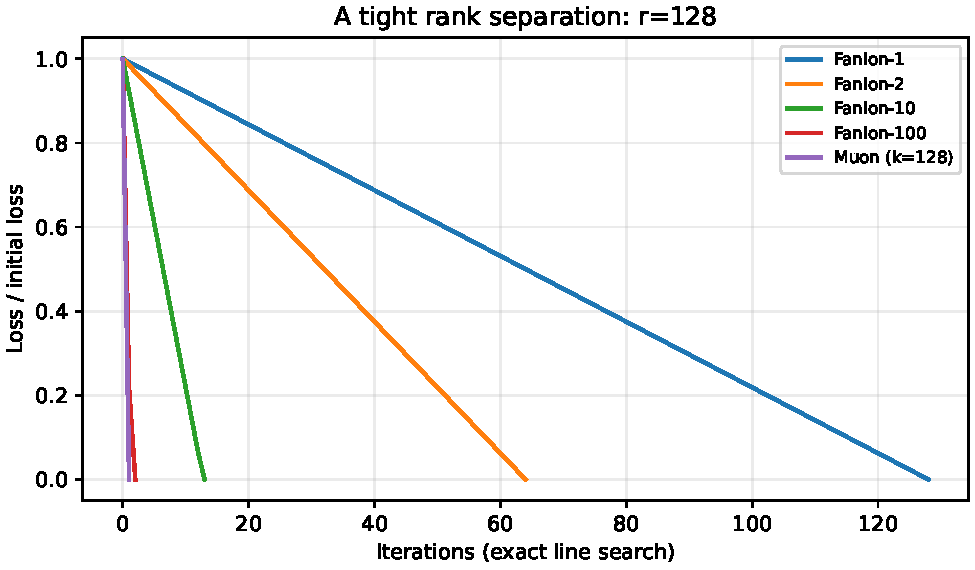
\includegraphics[width=0.73\linewidth]{results/rank_barrier.pdf}
\caption{Exact line-search trajectories attaining the rank obstruction.
This is an explanatory quadratic, not the manuscript's random instance.}
\end{figure}

\subsection{What hybrids change}

For $H\ne0$, the F-Fanion singular vectors are shared by its two summands, so
\[
 \nuc{D_{F,k}(H)}=ak+b\frac{\nuc H}{\F H}\leq ak+b\sqrt r
\]
when $\rank H\geq k$. The S-Fanion satisfies
\[
 \nuc{D_{S,k}(H)}\leq ak+b\eta\sqrt{r\,mn}.
\]
Consequently \eqref{eq:nuclear-bound} holds for these methods with $k$ in
the step budget replaced by these respective upper bounds. Their updates
can have full rank, so \eqref{eq:rank-bound} with the original $k$ is no
longer available.

For $r=500$, $a=b=1/2$, the F-Neon capacity upper bound is about 11.68,
versus 1 for Neon and 500 for Muon. At $\gamma_F=0.015$, the same new draw
requires at least 2,604 F-Neon steps by this bound, versus 117 for F-Muon.
The rank floor disappears, but a large nuclear-budget difference remains.
The S bound is deliberately conservative because the nuclear norm of a sign
matrix depends on its orientation and sign pattern.

\paragraph{Scope with normalization and decay.}
The additive-iterate hypothesis holds for the synthetic runs, where
\path{code/L_smooth_tests/run_benchmarks_new.py} sets
\texttt{norm\_weight=False}. If $X_{t+1}=c_tX_t-\gamma_tA_t$, then
$X_T=(\prod_t c_t)X_0$ plus a low-rank sum with rescaled coefficients.
One must apply the rank comparison to $Z-(\prod_t c_t)X_0$, and account for
the products in the nuclear budget. The displayed bounds do not transfer
unchanged to CIFAR weight normalization or to arbitrary decay.

\section{Upper bounds retaining the gradient spectrum}\label{sec:angles}

Assume Frobenius $L$-smoothness:
\[
 f(X+Y)\leq f(X)+\ip{G}{Y}+\frac L2\F Y^2.
\]
For a nonzero descent direction $D$, define
\begin{equation}\label{eq:angle}
 q(G,D)=\frac{\ip{G}{D}^2}{\F G^2\F D^2}\in[0,1].
\end{equation}
The score is unchanged by positive scalar scaling of $D$. For an exact
Fanion with $\rank G\geq k$, it is
\begin{equation}\label{eq:qk}
 q_k(G)=\frac{S_k(G)^2}{k\F G^2}.
\end{equation}
For rank-deficient gradients, the same expression remains a conservative
quantity; the exact cosine uses $\min(k,\rank G)$ in the denominator.

\begin{theorem}[Spectrum-dependent descent and PL convergence]\label{thm:upper}
Use the true gradient and set
$\gamma_t=S_k(G_t)/(Lk)$. Then
\begin{equation}\label{eq:spectrum-descent}
 f(X_{t+1})\leq f(X_t)-\frac{S_k(G_t)^2}{2Lk}
 =f(X_t)-\frac{q_k(G_t)}{2L}\F{G_t}^2.
\end{equation}
In particular,
\begin{equation}\label{eq:trajectory}
 \sum_{t<T}q_k(G_t)\F{G_t}^2\leq2L(f(X_0)-f_*).
\end{equation}
If $q_k(G_t)\geq\underline q_k>0$ along the trajectory, then
$\min_{t<T}\F{G_t}^2\leq2L(f(X_0)-f_*)/(T\underline q_k)$.
If additionally $\F{\nabla f(X)}^2\geq2\mu(f(X)-f_*)$ along the trajectory,
then
\begin{equation}\label{eq:pl}
 f(X_T)-f_*\leq
 (1-\mu\underline q_k/L)^T(f(X_0)-f_*).
\end{equation}
\end{theorem}
\begin{proof}
Apply smoothness with $Y=-\gamma_tD_k(G_t)$ and use
\eqref{eq:fanion-identities}; if the active rank is smaller, $\F D^2\leq k$
still gives the stated inequality. Substitute the step size, telescope, and
then apply the respective lower bounds on $q_k$ and $\F{G_t}^2$.
\end{proof}

For a flat nonzero singular spectrum with $r$ modes, $q_k=k/r$.
Thus the upper bounds retain a factor $r/k$ in deterministic iterations,
and the PL rate is $O((L/\mu)(r/k)\log(\Delta/\epsilon))$ if this
flatness condition persists. A more robust sufficient assumption is
$\sigma_1/\sigma_r\leq\chi$, which gives
$q_k\geq k/(\chi^2r)$. This is a structural assumption to measure, not a
consequence of smoothness.

At a common matrix $G$, the exact Muon--Neon ratio is
\begin{equation}\label{eq:muon-neon}
 \frac{q_r(G)}{q_1(G)}
 =\frac1r\left(\frac{\nuc G}{\op G}\right)^2.
\end{equation}
The ratio ranges from $1/r$ to $r$. Muon's Frobenius decrease certificate is
larger precisely when $\nuc G/\op G>\sqrt r$.

\paragraph{Why a worst-case bound cannot rank them.}
In fact,
\[
 \inf_{G\ne0}\frac{S_k(G)^2}{k\F G^2}
 =\min\{1/k,k/r\}.
\]
To see this, express a decreasing nonnegative singular vector as a
nonnegative sum of the step vectors $v_j=(1,\ldots,1,0,\ldots,0)$.
After imposing $S_k=1$, it is a convex combination of
$v_j/\min(k,j)$. Convexity of the squared Euclidean norm gives its maximum
as $\max_j j/\min(k,j)^2=\max(1,r/k^2)$.
Rank-one and flat vectors attain the endpoints.
In particular, the worst-case constants for both Neon and Muon are $1/r$.
Additional spectrum or curvature information is mathematically necessary.

\paragraph{Upper certificates are not observed speedups.}
Equation~\eqref{eq:muon-neon} compares two certified decreases at the
\emph{same} point with separately optimized scalar steps. It does not bound
the ratio of their complete training times. Different algorithms visit
different points; a ratio of upper complexity bounds is not a lower bound
on their actual runtime ratio.

\section{F-Muon and S-Muon: explicit robustness bounds}

Take $H=G\ne0$ and $\rank G\geq k$, and put
$x=S_k(G)/\F G$, so that $x^2/k=q_k$.

\begin{proposition}[Exact F-hybrid formula]\label{prop:f}
For $a,b\geq0$, not both zero,
\begin{equation}\label{eq:fq}
 q_{F,k}=
 \frac{(ax+b)^2}{a^2k+b^2+2abx}\geq q_k.
\end{equation}
\end{proposition}
\begin{proof}
The numerator follows from $\ip{G}{D_{F,k}}=aS_k+b\F G$.
The denominator follows from
$\ip{D_k}{G/\F G}=x$.
After multiplying by the positive denominators, the difference from $q_k$
has numerator $(k-x^2)(2abx+b^2)\geq0$.
\end{proof}
Thus adding a positive normalized \emph{true} gradient can only improve the
Frobenius angle. This explains why F-Muon can improve upon Muon on the
synthetic task in this particular upper bound. It also proves that this
bound alone cannot explain a universal advantage of Muon over NSGD or
F-Neon: NSGD has angle one.

\begin{proposition}[S-hybrid retention]\label{prop:s}
For $a>0$, $b\geq0$, $\eta\geq0$, and $d_0=\#\{G_{ij}\ne0\}$,
\begin{equation}\label{eq:sq}
 q(G,D_{S,k})\geq
 \frac{q_k(G)}{(1+\rho_{S,k})^2},\qquad
 \rho_{S,k}=\frac{b\eta\sqrt{d_0}}{a\sqrt k}.
\end{equation}
\end{proposition}
\begin{proof}
$\ip{G}{D_{S,k}}=aS_k+b\eta\ent G\geq aS_k$, while
$\F{D_{S,k}}\leq a\sqrt k+b\eta\sqrt{d_0}$. Substitute in
\eqref{eq:angle}. No sign assumption on the cross term
$\ip{D_k}{\sgn(G)}$ is needed.
\end{proof}

For F-Muon with $a=b=1/2$, the normalized-gradient component has Frobenius
length only $1/\sqrt r$ of the Muon component. For full-rank S-Muon on a
dense matrix, the corresponding relative length is
$\eta\sqrt{\max(m,n)}$. Thus the raw coefficient $\alpha=1/2$ does not mean
equal contribution to the actual update length.
For the saved CIFAR shapes and $\eta=0.003$, \eqref{eq:sq} preserves between
76.4\% and 91.7\% of the Muon angle certificate. These are uniform
worst-case retentions, not predicted validation accuracies.

More generally, for a PSD curvature majorant $\mathcal H$ and
$D=aD_0+bD_1$ with $\ip{G}{D_1}\geq0$, the curvature score in the next
section retains at least $(1+\rho)^{-2}$ of that of $D_0$, where
$\rho=b\F{\mathcal H^{1/2}D_1}/(a\F{\mathcal H^{1/2}D_0})$.
Here the notation denotes the norm on the vectorized matrix space.

\section{Curvature: the comparison that can account for reversals}

Suppose a quadratic upper model is valid along the considered step:
\begin{equation}\label{eq:curv-upper}
 f(X-\gamma D)\leq f(X)-\gamma A+\frac{\gamma^2}{2}C(D),\qquad
 A=\ip{G}{D},\quad C(D)>0.
\end{equation}
For example, $C(D)=\ip{D}{\mathcal HD}$ if
$\nabla^2 f\preceq\mathcal H$ on the segment. The optimized decrease
certificate is
\begin{equation}\label{eq:curv-score}
 \frac12\mathcal I(G,D),\qquad
 \mathcal I(G,D)=\frac{\pos A^2}{C(D)},\quad
 \gamma=\frac{\pos A}{C(D)}.
\end{equation}
If the model is only valid up to a maximal step, truncate $\gamma$ and use
\eqref{eq:curv-upper} directly. For a quadratic, the model is exact at every
step, so this is the \emph{actual} optimal one-step decrease.

For \eqref{eq:quadratic},
\begin{equation}\label{eq:quad-curv}
 C(D)=\ip{D}{MDN}=\F{M^{1/2}DN^{1/2}}^2.
\end{equation}
Writing $u_i,v_i$ for the singular vectors of $G$, the Fanion curvature is
\[
 C(D_k)=\sum_{i,j\leq k}
  (u_i^\top M u_j)(v_i^\top N v_j).
\]
The cross terms matter. Replacing this by $Lk$ may obscure the correct
ordering. In particular, at a common point Muon's curvature score beats
Neon's exactly when
\begin{equation}\label{eq:curvature-condition}
 \left(\frac{\nuc G}{\op G}\right)^2>
 \frac{C(D_r)}{C(D_1)}.
\end{equation}
This is a directly testable condition. Under the Frobenius majorant it
reduces to the threshold in \eqref{eq:muon-neon}.

\subsection{An explicit structured quadratic with the desired ordering}

Take $m=n=r$, $N=I$, $M=\Lambda=\operatorname{diag}(\lambda_i)\succ0$,
and $X_0=I$. The optimum of $f(X)=\ip{X}{\Lambda X}/2$ is zero, and
$G_0=\Lambda$. Muon's direction is $I$, so step one solves the problem.
Neon with exact line search only removes the diagonal entry with the
largest remaining $\lambda_i$, and requires exactly $r$ steps for zero
loss. Fanion-$k$ takes $\lceil r/k\rceil$. S-Muon is proportional to $I$
on this iterate, and likewise solves the problem in one step.

For F-Muon, choose step $1/a$ rather than even optimizing it. Then
\[
 \frac{f(X_1)}{f(X_0)}\leq
 \left(\frac ba\right)^2
 \frac{\sum_i\lambda_i^3}
 {\bigl(\sum_i\lambda_i^2\bigr)\bigl(\sum_i\lambda_i\bigr)}
 \leq \left(\frac ba\right)^2\frac{\kappa}{r},\quad
 \kappa=\frac{\lambda_{\max}}{\lambda_{\min}}.
\]
Hence, for bounded $\kappa$, F-Muon is close to the one-step optimum as
$r$ increases. This is a member of the manuscript's quadratic class with
a structured initialization, not a claim about all Gaussian initializations.

As a numerical illustration, for $r=128$ and log-spaced
$\lambda_i\in[0.001,1]$, exact line search gives:
\begin{center}
\begin{tabular}{lrr}\toprule
Direction & Frobenius angle $q$ & Remaining fraction of loss\\\midrule
Neon & 0.1031 & 0.947011\\
F-Neon & 0.6605 & 0.614410\\
NSGD & 1.0000 & 0.249105\\
Muon & 0.2868 & 0\\
F-Muon & 0.3531 & 0.006614\\
S-Muon & 0.2868 & 0\\\bottomrule
\end{tabular}
\end{center}
The curvature-aware calculation recovers the ordering even though the
Frobenius angles favor NSGD and F-Neon. This illustrates what information
is missing from a norm-only explanation.

\subsection{A counterexample to a universal Muon advantage}

For $f(X)=\F X^2/2$ at
$X=\operatorname{diag}(1,\delta,\ldots,\delta)$ with $\delta>0$, both
directions have full-rank gradient inputs, and exact line search gives
\[
 \frac{\text{Muon one-step decrease}}{\text{Neon one-step decrease}}
 =\frac{(1+(r-1)\delta)^2}{r}.
\]
At $r=64$, $\delta=0.001$, Neon has 56.64 times the one-step decrease.
Consequently smoothness, strong convexity, and exact gradients alone do
not imply the desired local ordering. A theorem imposing it in all cases
would be false.

\section{Stochastic gradients, momentum, and inexact LMOs}

The next result keeps the estimator error visible instead of assuming
orthogonalization of a stochastic matrix is unbiased.

\begin{theorem}[Oracle-input error]\label{thm:error}
Let $H=G+E$, and let $\widetilde D$ satisfy
\[
 \op{\widetilde D}\leq1,\quad\nuc{\widetilde D}\leq k,\qquad
 \delta=S_k(H)-\ip{H}{\widetilde D}\geq0.
\]
Then
\begin{equation}\label{eq:input-error}
 \ip{G}{\widetilde D}\geq S_k(G)-2S_k(E)-\delta,
 \qquad \F{\widetilde D}^2\leq k.
\end{equation}
Thus an $L$-smooth objective obeys
\begin{equation}\label{eq:noisy-decrease}
 f(X-\gamma\widetilde D)\leq f(X)
 -\gamma S_k(G)+2\gamma S_k(E)+\gamma\delta+L\gamma^2k/2.
\end{equation}
\end{theorem}
\begin{proof}
The support function of
$\{D:\op D\leq1,\nuc D\leq k\}$ is $S_k$.
Thus $\ip{G}{\widetilde D}\geq S_k(H)-\delta-S_k(E)$.
Use the triangle inequality $S_k(H)\geq S_k(G)-S_k(E)$.
Also $\F{\widetilde D}^2\leq\op{\widetilde D}\nuc{\widetilde D}\leq k$.
Apply smoothness for the last assertion.
\end{proof}

For an arbitrary momentum matrix, take $H$ to be any positive rescaling
of the \emph{actual} oracle input; $E=H-G$ then contains both noise and
tracking bias. For an approximate Newton--Schulz update outside the
feasible set, the feasibility and $\F{\widetilde D}^2\leq k$ claims cannot
be assumed: use the actual direction and its norm in
\eqref{eq:curv-upper}, or control its violation separately.

\subsection{An explicit sample bound with minibatches}

Use the normalized Frobenius step $X_{t+1}=X_t-hD_k(H_t)/\sqrt k$.
Suppose $q_k(G_t)\geq\underline q>0$ almost surely and
\[
 \E S_k(H_t-G_t)/\sqrt k\leq\nu_k/\sqrt B,
\]
with exact LMOs. Writing $\Delta=f(X_0)-f_*$, telescoping
\eqref{eq:noisy-decrease} yields
\begin{equation}\label{eq:batch-bound}
 \frac1T\sum_{t<T}\E\F{G_t}\leq
 \frac{1}{\sqrt{\underline q}}
 \left(\frac{\Delta}{hT}+\frac{Lh}{2}
       +\frac{2\nu_k}{\sqrt B}\right).
\end{equation}
For $h=\sqrt{2\Delta/(LT)}$, it suffices to choose
\[
 T\geq\frac{8L\Delta}{\underline q\epsilon^2},\qquad
 B\geq\frac{16\nu_k^2}{\underline q\epsilon^2}
\]
to make the left side at most $\epsilon$. Rounding to positive integers
gives total gradient evaluations of order
\[
 \left(1+\frac{L\Delta}{\underline q\epsilon^2}\right)
 \left(1+\frac{\nu_k^2}{\underline q\epsilon^2}\right).
\]
The exponent four in the noise-dominated term remains, but its coefficient
retains $1/\underline q^2$ and the projected noise $\nu_k^2$.
Under a common Frobenius variance bound $\E\F{H_t-G_t}^2\leq\sigma^2/B$,
one may conservatively take $\nu_k=\sigma$. The flat-spectrum condition
then gives rank factors $r/k$ and $(r/k)^2$ in these sufficient iteration
and sample bounds. Those are comparisons of certificates under the
stated trajectory conditions, not proved time ratios between arbitrary
stochastic training runs.

\subsection{A fixed-batch momentum bound with the same spectral factor}

For clarity, this calculation is for EMA heavy ball, not the implemented
Nesterov variant. Let $m_{-1}=0$, $\alpha=1-\beta\in(0,1]$,
$m_t=\beta m_{t-1}+\alpha g_t$, and
$X_{t+1}=X_t-hD_k(m_t)/\sqrt k$. Assume conditionally unbiased
$g_t=G_t+\xi_t$ with conditional Frobenius variance at most $\sigma^2$,
and $q_k(G_t)\geq\underline q$.
Then
\begin{equation}\label{eq:ema-bound}
\begin{split}
 \frac1T\sum_{t<T}\E\F{G_t}\leq\frac1{\sqrt{\underline q}}
 \bigg(&\frac{\Delta}{hT}+\frac{Lh}{2}
 +\frac{2\beta\F{G_0}}{\alpha T}
 +\frac{2\beta Lh}{\alpha}
 +2\sigma\sqrt{\frac{\alpha}{2-\alpha}}\bigg).
\end{split}
\end{equation}
To verify this, unroll
\[
 m_t-G_t=-\beta^{t+1}G_0+
 \sum_{s=1}^t\beta^{t-s+1}(G_{s-1}-G_s)
 +\alpha\sum_{s=0}^t\beta^{t-s}\xi_s.
\]
The drift norm is at most $\beta Lh/\alpha$ because each iterate moves
by at most $h$. Martingale orthogonality bounds the last term's expected
norm by $\sigma\sqrt{\alpha/(2-\alpha)}$. Average the initial term,
apply Theorem~\ref{thm:error}, and telescope.

Taking $\alpha$ of order
$\min(1,\underline q\epsilon^2/\sigma^2)$ and
$h$ of order $\epsilon\sqrt{\underline q}\alpha/L$, with sufficiently
small constants, gives the sufficient complexity
\begin{equation}\label{eq:ema-complexity}
 T=O\!\left(1+
 \frac{L\Delta}{\underline q\epsilon^2}
 +\frac{L\Delta\sigma^2}{\underline q^2\epsilon^4}
 +\frac{\F{G_0}}{\sqrt{\underline q}\epsilon}
 +\frac{\F{G_0}\sigma^2}{\underline q^{3/2}\epsilon^3}\right).
\end{equation}
This displays the finite-precision terms as well as the fourth-power
asymptotic term. It is a straightforward specialization of standard
tracking arguments, not a claim to improve the universal stochastic
first-order exponent.

\section{Audit of the repository's CIFAR gradient logs}\label{sec:audit}

The script analyzes the predeclared cohort
\path{code/cifar_norms/grad_norms_*_run0_20251208_*.csv}:
nine trajectories, all 250 logged steps in each, all six trained convolution
matrices, totaling 13,500 layer snapshots. Shapes are inferred from
\texttt{CifarNet} in \path{code/cifar_bench/norm_logger_airbench.py}:
$64\times216$, $64\times576$, $256\times576$, and three
$256\times2304$ matrices. The CSVs themselves do not store shape metadata.

The following table uses the Muon trajectory as a common collection of
matrices, not a comparison of different stopping norms. The same diagnostic
is also output for all other trajectories.
\begin{center}\small
\begin{tabular}{lrrrrr}
\toprule
Layer & $r$ & median $q_r/q_1$ & $\Pr(q_r>q_1)$ & median $q_{F,r}/q_r$ & median $q_{F,1}/q_r$ \\
\midrule
1.conv1 & 64 & 1.67 & 88.0\% & 1.17 & 1.62 \\
1.conv2 & 64 & 2.84 & 98.4\% & 1.10 & 1.13 \\
2.conv1 & 256 & 2.81 & 97.2\% & 1.10 & 1.55 \\
2.conv2 & 256 & 3.81 & 97.2\% & 1.07 & 1.25 \\
3.conv1 & 256 & 1.94 & 89.6\% & 1.10 & 1.63 \\
3.conv2 & 256 & 2.10 & 96.0\% & 1.14 & 2.08 \\
\bottomrule
\end{tabular}

\end{center}
Here $\Pr$ denotes the fraction of logged snapshots, not a statistical
population probability or a confidence interval. $a=b=1/2$ for both F
columns. The $q$ values are computed from the three saved norms using
\eqref{eq:qk} and \eqref{eq:fq}.

\paragraph{Positive finding.}
The median Muon--Neon ratio is between 1.67 and 3.81 across the six layers,
and favors Muon in 88.0--98.4\% of snapshots. Hence the observed spectra
are broadly compatible with a better Muon descent certificate.

\paragraph{Negative finding that limits the conclusion.}
The F-Neon--Muon surrogate ratio has median 1.13--2.08, favoring F-Neon.
Yet F-Neon is empirically weaker. Therefore these spectra and a common
Frobenius smoothness constant do \emph{not} suffice to explain the complete
ranking. Curvature, actual momentum alignment, and finite learning-rate
budgets must be retained. F-Neon also has a much smaller update length at
the manuscript's inherited learning rate than an independently rescaled
angle comparison permits.

\paragraph{Data limitations.}
The CSVs store raw minibatch gradient norms, not the full population gradient,
the momentum input, exact singular vectors, Hessian products, or update
matrices. A nonlinear map of a stochastic gradient is not generally an
unbiased map of the true gradient. Moreover, the reference Muon file has
only 8 finite loss entries out of 250, although all the norm entries used
here are finite. We do not fit loss rates to that column, infer the cause
of its nonfinite entries, or use this cohort's final accuracy as the
manuscript's eight-epoch result. Source filenames, hashes, counts, and
finite-loss counts are saved in \path{results/summary.json}.

\begin{figure}[ht]
\centering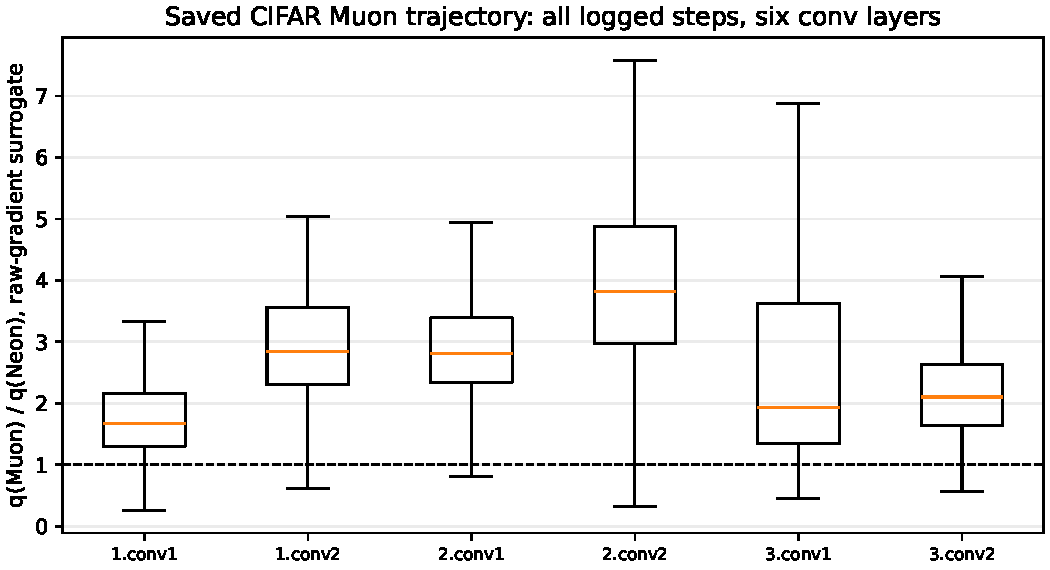
\includegraphics[width=0.91\linewidth]{results/cifar_diagnostics.pdf}
\caption{Muon--Neon Frobenius certificate ratios from the same saved raw
gradient matrices. Boxes summarize the reference trajectory; they are not
measured speedups or convergence rates.}
\end{figure}

\section{How to turn the conditional part into an experimental explanation}

The missing measurements are specific and considerably smaller than a full
Hessian. On common saved checkpoints and fixed evaluation batches:
\begin{enumerate}
\item Save the actual oracle input $H_t$ and the actual update matrix for
each method, including Newton--Schulz approximation and scaling. Use a
shared large-batch evaluation gradient $G_t$ to measure
$\ip{G_t}{D_t}$ and the error $H_t-G_t$ after an appropriate positive
rescaling of $H_t$.
\item Measure $\ip{D_t}{\nabla^2 f(X_t)D_t}$ with one Hessian--vector product
per candidate direction, or use central loss differences at several small
steps. On a nonconvex neural network a pointwise Hessian value is only a
local estimate; verify the quadratic upper model at the actual step, rather
than calling that value a global smoothness constant.
\item Compare $\gamma_t\ip{G_t}{D_t}-\gamma_t^2 C_t(D_t)/2$ at the actual
learning rate and $\mathcal I(G_t,D_t)$ at a separately optimized step.
This separates a finite step-budget limitation from a directional curvature
limitation. With multiple layers, include cross-layer curvature or justify
a block-diagonal upper model before adding per-layer certificates.
\item For the quadratic, compute $E_0$ from the original saved $M,N,X_0$ and
substitute its singular values into Theorem~\ref{thm:barriers}. This yields
a bound on the original run without a new optimizer sweep.
\end{enumerate}

\path{analyze.py --snapshot example.npz} already computes the exact
projections and, when the NPZ contains \texttt{left} and \texttt{right},
the exact quadratic curvature scores. It accepts \texttt{oracle\_input}
separately from \texttt{gradient}; therefore it does not silently equate
the raw gradient with a Nesterov direction.

\section{Implementation and manuscript details discovered during the check}

These observations are recorded here; no original source was edited.
\begin{enumerate}
\item Equation \texttt{eq:ckfk\_norm} in the manuscript puts
$(1-\alpha)/\eta$ before the entrywise $\ell_1$ norm, while its update uses
$(1-\alpha)\eta\sgn(H)$. The support function of the actual Minkowski-sum
ball is $\alpha S_k(H)+(1-\alpha)\eta\ent H$. Thus that equation's
coefficient should be $(1-\alpha)\eta$ to match the displayed update.
\item The manuscript defines a normalized EMA buffer
$B_t=\beta B_{t-1}+(1-\beta)g_t$ and approximate Nesterov input $g_t+\beta B_t$.
\path{code/optimizers.py} accumulates $b_t=\beta b_{t-1}+g_t$ and uses
$g_t+\beta b_t$. With $B_t=(1-\beta)b_t$, the code input is
$g_t+\beta B_t/(1-\beta)$. The two mixtures are generally not positive
scalar multiples, unlike the heavy-ball case. Theory should specify which
one is being analyzed.
\item The Frobenius smoothness constant of the quadratic is
$L=\op M\op N$. Some helper expressions in
\path{code/L_smooth_tests/problems.py} use other, looser quantities.
The obstruction proved here uses the exact Frobenius constant and does
not rely on those helper expressions.
\end{enumerate}

\section{Reproduction and conclusion}

From the repository root, run
\begin{verbatim}
python theory_attempts/analyze.py
python theory_attempts/build_report.py
\end{verbatim}
The supplied PDF and standalone HTML use Pandoc's MathML export and a
headless browser, keeping browser profiles in this folder. This avoids
the current sandbox's MiKTeX initialization failure. For a normal LaTeX
build instead, use:
\begin{verbatim}
cd theory_attempts
pdflatex -interaction=nonstopmode -halt-on-error bounds.tex
pdflatex -interaction=nonstopmode -halt-on-error bounds.tex
\end{verbatim}
The Python script uses NumPy and Matplotlib on CPU and writes only to
\path{theory_attempts/results}. The run checked 160 random rectangular cases
for each angle/oracle assertion, 800 exact quadratic decrease identities,
and 640 trajectory points for each quadratic lower bound. The largest
relative error in the quadratic identities was below $1.5\cdot10^{-15}$.
These numerical checks complement the proofs; they do not prove theorems
or validate assumptions on neural-network trajectories.

\paragraph{Answer to the research question.}
Yes, there are substantially more discriminating bounds than a common
$O(\epsilon^{-4})$ statement: a rigorous finite-step explanation of Neon's
slow progress on the synthetic class, a tight $r/k$ separation example,
and spectrum/curvature/noise-dependent upper bounds with explicit hybrid
robustness. The quadratic obstruction is ready to use after substituting
the original instance's spectrum. A complete quantitative explanation of
the CIFAR/LLM ordering remains open in this attempt because the required
curvature and momentum measurements are absent. The existing log audit
shows exactly where a simpler explanation succeeds and where it fails.

\begin{thebibliography}{9}
\bibitem{structured} D. Kovalev and E. Borodich.
\emph{Non-Euclidean SGD for Structured Optimization: Unified Analysis and
Improved Rates}, v2, 2026.
\url{https://arxiv.org/html/2511.11466v2}.
\bibitem{shen} W. Shen, R. Huang, M. Huang, C. Shen, and J. Zhang.
\emph{On the Convergence Analysis of Muon}, v3, 2026.
\url{https://arxiv.org/html/2505.23737v3}.
\bibitem{nagashima} S. Nagashima and H. Iiduka.
\emph{Improved Convergence Rates of Muon Optimizer for Nonconvex Optimization},
v3, 2026. \url{https://arxiv.org/html/2601.19400v3}.
\bibitem{schattor} B. Ma, J. Zhang, and C. He.
\emph{Schattor: Schatten-family methods for deep learning optimization},
2026. Abstract checked at \url{https://arxiv.org/abs/2606.15702}.
\bibitem{trust} D. Kovalev.
\emph{Understanding Gradient Orthogonalization for Deep Learning via
Non-Euclidean Trust-Region Optimization}, v2, 2025.
\url{https://arxiv.org/html/2503.12645v2}.
\bibitem{gluon} A. Riabinin, E. Shulgin, K. Gruntkowska, and P. Richtarik.
\emph{Gluon: Making Muon \& Scion Great Again!}, 2025.
\url{https://arxiv.org/html/2505.13416}.
\end{thebibliography}
\end{document}
